
\documentclass[a4paper,11pt]{article}

\usepackage[spanish, activeacute]{babel}
\usepackage[ansinew]{inputenc}
\usepackage{graphicx}

\renewcommand{\labelitemii}{\Radioactivity}

%PSUDO

% PSEUDOCODIGO
\newcounter{linea}
\newenvironment{pseudo}{
	\setcounter{linea}{0}
    \begin{small}
    \begin{tt}
    \begin{tabbing}
        ------ \= ---- \= ---- \= ---- \= ---- \= ---- \= ---- \kill
} {
    \end{tabbing}
    \end{tt}
    \end{small}
}

\newcommand{\n}{
    \addtocounter{linea}{1}
    \arabic{linea}.
}

\newcommand{\tab}{\>}
%END PSEUDO
\begin{document}

\markboth{left head}{KANON dbms Operations manual } \pagestyle{myheadings} 

\title{
	\mbox{\Huge Base de Datos}\\
	%\mbox{\Huge Trabajo Pr�ctico Final}\\
	\mbox{}\\
	\mbox{\it Implementaci�n de algoritmo de ARIES }\\
	\mbox{\it sobre desarrollo de DBMS}\\
	\mbox{}\\
	Departamento de Computaci�n \\
	Facultad de Ciencias Exactas y Naturales\\
	Universidad de Buenos Aires
\date{}
}
\maketitle
\begin{center}
	\begin{tabular}{cc}
		Luciano Leggieri&Julian Berl�n\\
		{\small \verb"lleggieri@dc.uba.ar"}&{\small \verb"jberlin@dc.uba.ar"}\\
		\cr
		Victor Cabas&Facundo Pippia\\
		{\small \verb"vcabas@dc.uba.ar"}&{\small \verb"facundomensajes@hotmail.com"}\\
	\end{tabular}
	\vskip 5 mm
	Director:\\
	Alejandro Eidelsztein\\
	{\small \verb"ae0n@dc.uba.ar"}\\
\end{center}

{\centering {\bf Abstract}\\}
ARIES es un algoritmo de recuperaci�n muy popular que usa un enfoque steal / no-force. Comparado con otros esquemas de recuperaci�n, es simple y soporta diferentes grados de granularidad en los bloqueos. Luego de una ca�da, este algoritmo procede en tres fases para dejar la base de datos en el estado que tenia antes del crash. El objetivo de este trabajo es realizar una implementaci�n de ARIES en un motor de base de datos construido �ntegramente en Java. 

\vskip 5 mm

\texttt{Keywords: Bases de datos relacionales, ARIES, Transacciones, Recovery Manager}
\newpage
\tableofcontents
\newpage
\listoffigures
\newpage

\section{Requisitos del Sistema}

Tanto el cliente como el servidor fueron hechos en la plataforma Java SE versi�n 5. El runtime de la misma es necesario para poder ejecutarlos, y los programas funcionar�n en cualquier sistema que cumpla con los requisitos del runtime (x86, x64 o PowerPC; ha sido probado en Windows, Linux y Mac OSX). La maquina virtual se puede conseguir de www.java.com\\

\section{Ejecuci�n de los programas}

Para correr al servidor y al cliente se disponen de respectivos programas batch que se encargan de levantarlos.\\

Para el servidor, el archivo a ejecutar es \textbf{servidor.bat} dentro del directorio \textbf{kanon-server}.\\

Para el cliente, el archivo es \textbf{cliente.bat} dentro del directorio \textbf{kanon-cliente}.\\

Para bajar el servidor, se debe ejecutar el archivo \textbf{stop.bat} dentro del directorio \textbf{kanon-server}.\\

\section{Par�metros de configuraci�n disponibles}

En el servidor, a trav�s de par�metros pasados en la ejecuci�n del batch, se puede modificar la configuraci�n inicial del motor. Los par�metros se pasan de la forma:\\
\textbf{\textit{-Dparam=valor}}

Los par�metros soportados son los siguientes:\\

\textbf{pool:} toma como valor un n�mero que indica la cantidad de slots disponibles para paginas que tendr� el Buffer Manager. Por omisi�n son 8.

\textbf{politica:} indica el algoritmo de remoci�n utilizado en el Buffer Manager cuando no quedan slots libres. Los valores pueden ser: \textbf{LRU}, \textbf{MRU}, \textbf{LFU}, \textbf{MFU}, \textbf{Azar}, \textbf{LIFO}, \textbf{FIFO}. Por omisi�n se toma LRU. Las opciones son case-sensitive.

\textbf{prevencion:} indica el algoritmo de prevenci�n de deadlock utilizado por el Lock Manager. Los valores disponibles son: \textbf{CautionWaiting}, \textbf{WaitDie}, \textbf{WoundWait}, \textbf{Nulo}. Por omisi�n se toma CautionWaiting. Como el anterior, las opciones son case-sensitive.


\section{Arquitectura, dise�o y especificaci�n del cliente}

Con el objetivo de poder testear y verificar el correcto funcionamiento del motor de base de datos construido, pensamos en el desarrollo de una herramienta cliente cuya principal funcionalidad iba ser poder verificar que efectivamente est�bamos haciendo las cosas bien y que el motor de base de datos funciona correctamente.\\

Sus principales caracter�sticas son las siguientes:\\
\begin{enumerate}
	\item Poder enviar consultas al servidor y verificar que el servidor las ha procesado correctamente.

	\item Hacer pruebas de concurrencia sobre el motor, es decir poder ejecutar m�s de una consulta de manera simult�nea.

	\item Observar que la implementaci�n de ARIES es correcta y funciona bien.

	\item Observar los locks y el valores que se insertan en el LOG.

	\item Poder simular un crash y ver como funciona la recuperaci�n.
\end{enumerate}


La arquitectura de alto nivel del cliente se resume en la siguiente figura:

\begin{figure}[h]
		\centering
		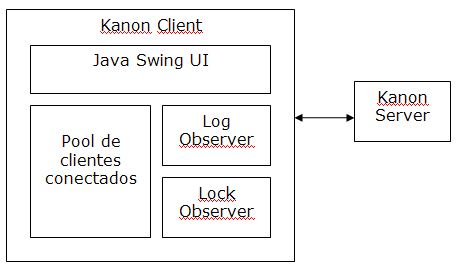
\includegraphics[scale=0.6]{img/arquitectura.png}
		\label{fig:arquitectura.png}
		\caption{Arquitectura del cliente}
\end{figure}

A continuaci�n se describe la funcionalidad de cada uno de los componentes\\
 
\begin{itemize}
	\item \textbf{Java Swing UI: }B�sicamente es el paquete de clases que usamos para construir la capa de presentaci�n del cliente, la versi�n de swing que usamos es la que viene con Java 5.

	\item \textbf{Pool de clientes conectados: }Es un objeto contenedor que almacena todos los clientes que est�n conectados con el motor.

	\item \textbf{Log Observer: }Es proceso que se encargar de estar todo el tiempo leyendo el log, se ejecuta como un thread aparte, �sea como un subproceso del cliente

	\item \textbf{Lock Observer: }Es proceso que se encarga de estar todo el tiempo leyendo la tabla de locks, se ejecuta como un thread aparte, o sea como un subproceso del cliente al igual que el log observer.
\end{itemize}

El esquema usado para conectarse con el servidor es el cl�sico client-server, a trav�s de sockets. Al agregarse un cliente, lo primero que se hace es crear un nuevo socket; el siguiente diagrama de secuencia muestra como se crea un cliente y se agrega al pool de clientes conectados:\\

 
\begin{figure}[h]
		\centering
		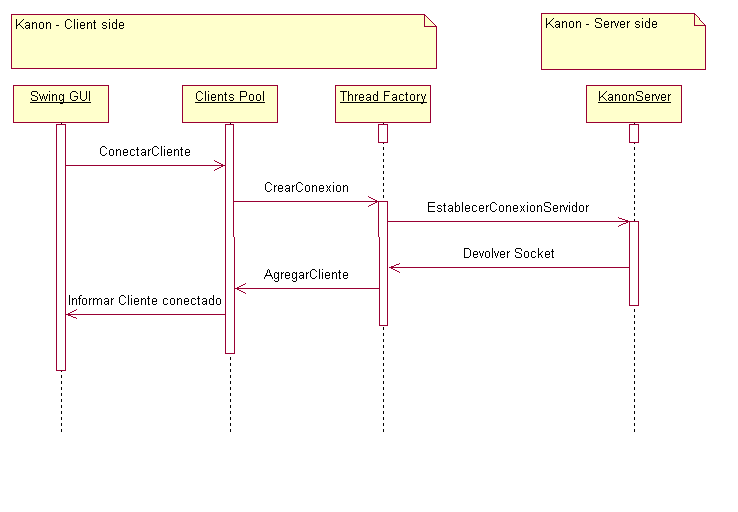
\includegraphics[scale=0.5]{img/secuencia.png}
		\label{fig:secuencia.png}
		\caption{Diagrama de secuencia de la ejecuci�n de una consulta}
\end{figure}

Cabe destacar que solo se podr� agregar un cliente al pool de clientes si es posible establecer una conexi�n con el servidor, de lo contrario no se podr� agregar.\\

\begin{figure}[h]
		\centering
		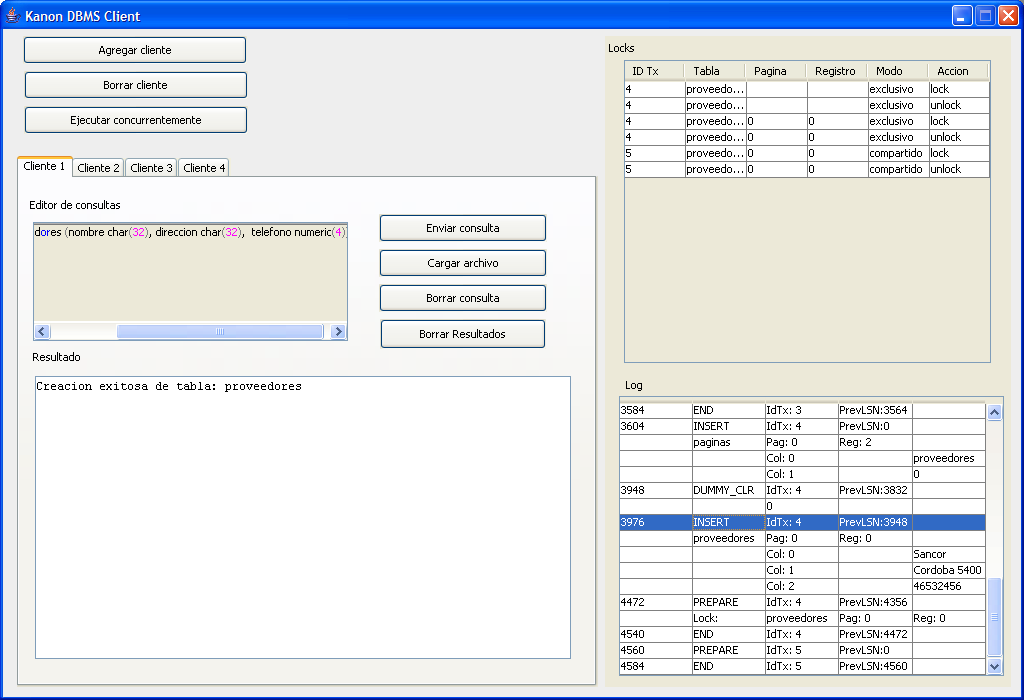
\includegraphics[scale=0.35]{img/cliente.png}
		\label{fig:cliente.png}
		\caption{Captura de pantalla del cliente en funcionamiento}
\end{figure}

Los botones disponibles son:\\
\begin{itemize}
	\item \textbf{Agregar cliente}: Crea una nueva conexi�n al servidor para enviar consultas.

	\item \textbf{Borrar cliente:} Borra a un cliente creado.

	\item \textbf{Ejecutar concurrentemente:} Lanza a la vez las consultas escritas en todos los clientes abiertos.
\end{itemize}

Y para cada cliente:\\
\begin{itemize}
	\item \textbf{Enviar consulta:} Env�a la consulta escrita al servidor y aguarda el resultado.

	\item \textbf{Cargar archivo:} Carga una consulta desde un archivo de texto y la coloca en el cuadro del editor de consultas.

	\item \textbf{Borrar consulta:} Limpia el contenido del editor de consultas.

	\item \textbf{Borrar resultados:} Limpia el contenido de la pantalla de resultados.
\end{itemize}


\section{Sentencias SQL soportadas}

Las siguientes plantillas de sentencias SQL son las soportadas por el servidor:\\
\\
\textbf{INSERT INTO tabla (col1, col2...) VALUES (valor1, valor2...);}\\
Inserta en una tabla una fila con los valores especificados.\\
\\
\textbf{INSERT INTO tabla (col1, col2...) SELECT...;}\\
Inserta en una tabla el resultado de la consulta dentro del SELECT.\\
\\
\textbf{UPDATE tabla SET col1 = expresion WHERE expresionWhere;}\\
Actualiza los registros de la tabla que cumplan con la condicion del Where a los valores especificados.\\
\\
\textbf{SELECT col1, expresion1... FROM tabla WHERE expresionWhere;}\\
Retorna los resultados de la tabla que cumplan con la condicion del Where.\\
\\
\textbf{DELETE FROM tabla WHERE expresionWhere;}\\
Borra de la tabla a aquellos registros que cumplan con la condicion del Where.\\
\\
\textbf{CREATE TABLE tabla (col1 NUMERIC/CHAR(XX)...);}\\
Crea una nueva tabla en el sistema, con las columnas especificadas. Los tipos disponibles son NUMERIC(4) y CHAR(vv) donde vv es el tama�o maximo de caracteres en la columna.\\
\\
\textbf{DROP TABLE tabla;}\\
Borra una tabla del sistema.\\
\\
\textbf{BEGIN TRANSACTION;}\\
Inicia una transacci�n explicita, o una transacci�n anidada si ya habia una en curso.\\
\\
\textbf{COMMIT TRANSACTION;}\\
Realiza un commit de la transacci�n en curso. Contin�a con la transacci�n padre en caso de existir una.\\
\\
\textbf{SAVEPOINT nombre;}\\
Guarda un savepoint de la posicion actual de la transaccion en curso. Si ya exist�a un savepoint con ese nombre, es sobrescrito.\\
\\
\textbf{ROLLBACK nombre;}\\
Realiza un rollback de la transacci�n en curso hasta el savepoint especificado. No termina la transacci�n.
\\
\textbf{ROLLBACK TRANSACTION;}\\
Realiza un rollback de toda la transacci�n en curso. Contin�a con la transacci�n padre en caso de existir una.\\
\\
\textbf{CRASH;}\\
Comando especial para simular una ca�da del sistema con fines educativos. Detiene el servidor. Se recomienda cerrar el cliente luego de esta operaci�n.\\
\\
\textbf{CHECKPOINT;}\\
Realiza un checkpoint en la base de datos, para acortar el tiempo necesario para realizar una recuperaci�n en caso de una ca�da del sistema. Al bajar el servidor se realiza un checkpoint autom�ticamente.\\
\\
\textbf{ISOLATION nivelAislamiento;}\\
Establece el nivel de aislamiento para las futuras transacciones. Los valores posibles son:
\textit{READ\_UNCOMMITTED}, \textit{READ\_COMMITTED}, \textit{REPEATABLE\_READ}, \textit{SERIALIZABLE.}\\


\end{document}
